\documentclass{beamer}
\mode<presentation> {\usecolortheme{wolverine}}
\usepackage{textgreek}
\usepackage{graphicx}
\usepackage{wrapfig}
\usepackage{graphicx}
\usepackage{bussproofs}
\usepackage{cspsym}
\usepackage{fancyvrb}
\usepackage{natbib}
\usepackage{color}
\usepackage{bbm}
\usepackage[greek,english]{babel}
\usepackage{ucs}
\usepackage[utf8x]{inputenc}
\usepackage{autofe}
\usepackage{tikz}
\usepackage{amssymb}
\usepackage{bbm}
\usepackage[greek,english]{babel}
\usepackage{ucs}
\usepackage[utf8x]{inputenc}
\usepackage{autofe}
\usepackage{fancyvrb}


\usepackage{setspace} 
\usepackage{makeidx}
\usepackage{graphicx}

\usepackage{amssymb,amsmath}
\usepackage{fancyvrb}
\usepackage[english]{babel}
\usepackage{natbib}
\usepackage{wrapfig}
\usepackage{ifpdf}
\usepackage{color}
\newcommand{\easychair}{\textsf{easychair}}
\newcommand{\miktex}{MiK{\TeX}}
\newcommand{\texniccenter}{{\TeX}nicCenter}
\newcommand{\makefile}{\texttt{Makefile}}
\newcommand{\latexeditor}{LEd}

\newcommand{\prefixoperator}{\mathbin{\mathord{\mbox{---}}\mathord{>}}}
\makeindex


\newcommand{\ar}{\rightarrow}
\newcommand{\all}{\forall}
%\newcommand{\binding}{\mathbin{\mathord{>}\hspace{-0.35em}\mathord{>}\hspace{-0.35em}\mathord{=}}}
\newcommand{\binding}{\gg}



\newcommand{\IO}{\mathsf{IO}}
\newcommand{\datarm}{\mathsf{data}}
\newcommand{\wheresf}{\mathsf{where}}
\newcommand{\conssf}{\mathsf{cons}}
\newcommand{\Set}{\mathsf{Set}}
\newcommand{\zrm}{\mathsf{z}}
\newcommand{\srm}{\mathsf{s}}
\newcommand{\Nbb}{\mathbb{N}}
\newcommand{\Streamsf}{\mathsf{Stream}}
\newcommand{\idsf}{\mathsf{id}}
\newcommand{\Msf}{\mathsf{M}}
\newcommand{\returnsf}{\mathsf{return}}
\newcommand{\record}{\mathsf{record}}
\newcommand{\mutual}{\mathsf{mutual}}
\newcommand{\Size}{\mathsf{Size}}
\newcommand{\coinductive}{\mathsf{coinductive}}
\newcommand{\constructor}{\mathsf{constructor}}
\newcommand{\delay}{\mathsf{delay}}
\newcommand{\field}{\mathsf{field}}
\newcommand{\force}{\mathsf{force}}
\newcommand{\ProcessShape}{\mathsf{ProcessShape}}
\newcommand{\Process}{\mathsf{Process}}
\newcommand{\Processplus}{\mathsf{Process}\mathord{+}}
\newcommand{\Choice}{\mathsf{Choice}}
\newcommand{\Lab}{\mathsf{Lab}}
\newcommand{\List}{\mathsf{List}}
\newcommand{\ChoiceSet}{\mathsf{ChoiceSet}}
\newcommand{\Label}{\mathsf{Label}}
\newcommand{\node}{\mathsf{node}}
\newcommand{\terminate}{\mathsf{terminate}}


\newcommand{\emptyhat}{\widehat{\emptyset}}
\newcommand{\tophat}{\widehat{\top}}
\newcommand{\efq}{\mathsf{efq}}
\newcommand{\Bool}{\mathrm{Bool}}
\newcommand{\Boolhat}{\widehat{\mathsf{Bool}}}
\newcommand{\plushat}{\mathbin{\widehat{+}}}
\newcommand{\IntChoice}{\mathsf{IntChoice}}
\newcommand{\ExtChoice}{\mathsf{ExtChoice}}
\newcommand{\deadlock}{\mathsf{deadlock}}
\newcommand{\fmap}{\mathsf{fmap}}
\newcommand{\inl}{\mathsf{inl}}
\newcommand{\inr}{\mathsf{inr}}
\newcommand{\Interrupt}{\mathsf{Interrupt}}
\newcommand{\hhide}{hide}
\newcommand{\Hide}{\mathsf{Hide}}
\newcommand{\ssubset}{\mathsf{subset}}
\newcommand{\projssubset}{\mathsf{projSubset}}
\newcommand{\interleaveop}{\mathbin{|||}}
\newcommand{\interleaveDef}{\mathord{\_|||\_}}

\newcommand{\with}{\mathsf{with}}
\newcommand{\Rename}{\mathsf{Rename}}
\newcommand{\parallelWithIndices}[2]{\mathbin{{}_{#1} \mathord{\parallel}{}_{#2}}}
\newcommand{\ff}{\mathsf{ff}}
\newcommand{\ttsf}{\mathsf{tt}}
\newcommand{\Parallelsf}{\mathsf{Parallel}}
\newcommand{\subsetsf}{\mathsf{subset}}
\newcommand{\Truesf}{\mathsf{True}}
\newcommand{\subsf}{\mathsf{sub}}

\newcommand{\emptyC}{\mathrm{empty}}
\newcommand{\extChoice}{\mathrm{trE}}
\newcommand{\intChoice}{\mathrm{trI}}
\newcommand{\Sym}{\mathrm{Sym}}
\newcommand{\Choi}{\mathrm{Choice}}
\newcommand{\Tr}{\mathrm{Tr}}

\newcommand{\pii}{\mathrm{PI}}
\newcommand{\pe}{\mathrm{PE}}
\newcommand{\ii}{\mathrm{I}}
\newcommand{\e}{\mathrm{E}}
\newcommand{\lab}{\mathrm{Lab}}
\newcommand{\subsett}{\mathrm{subset}}
\newcommand{\Subsett}{\mathrm{Subset}}

%\newcommand{\binding}{\mathbin{\mathord{>}\hspace{-0.35em}\mathord{>}\hspace{-0.35em}\mathord{=}}}







\newcommand{\includeXfigPictexWithoutFigure}[1]{\ifpdf
\begin{center}
\input #1.pdf_t
%\caption{Your figure}
\end{center}\else%
\begin{center}
\input #1.pstex_t
%\caption{Your figure}
\end{center}\fi}




\DeclareUnicodeCharacter{8988}{\ensuremath{\ulcorner}}
\DeclareUnicodeCharacter{8989}{\ensuremath{\urcorner}}
\DeclareUnicodeCharacter{8803}{\ensuremath{\overline{\equiv}}}





 \usepackage{amssymb}
 \usepackage{bbm}
 \usepackage[greek,english]{babel}

 \usepackage{ucs}
 \usepackage[utf8x]{inputenc}
 \usepackage{autofe}
\usepackage{graphicx} % Allows including images
\usepackage{booktabs} % Allows the use of \toprule, \midrule and \bottomrule in tables
%----------------------------------------------------------------------------------------
%	TITLE PAGE
%----------------------------------------------------------------------------------------

\title[Representing the Process Algebra CSP in Type
Theory]{Representing the Process Algebra CSP in Type
Theory} % The short title appears at the bottom of every slide, the full title is only on the title page

\author{Bashar Igried and Anton Setzer} % Your name
\institute[Swansea University] % Your institution as it will appear on the bottom of every slide, may be shorthand to save space
{
Swansea University, Swansea,Wales, UK \\ % Your institution for the title page
\medskip
\textit{bashar.igried@yahoo.com , a.g.setzer@swansea.ac.uk} % Your email address
}
\date{TYPES 2016, Novi Sad, Serbia, 26 May 2016} % Date, can be changed to a custom date

\begin{document}

% % % % % % % % % % % % % % % % % % % % % % % % % %

%Start document 

% % % % % % % % % % % % % % % % % % % % % % % % % %

\begin{frame}
\titlepage
\end{frame}


% % % % % % % % % % % % % % % % % % % % % % % % % %

%Over View 

% % % % % % % % % % % % % % % % % % % % % % % % % %




\begin{frame}
\frametitle{Overview}
\begin{enumerate}

\item Why Agda?
\item Process Algebra 
\item CSP
\item CSP-Agda
\item Choice Sets 
\item Future Work
\item Conclusion
 


\end{enumerate}
\end{frame}





% % % % % % % % % % % % % % % % % % % % % % % % % %

%Over View 

% % % % % % % % % % % % % % % % % % % % % % % % % %


%
%\begin{frame}
%\begin{itemize}
%
%\item Processes in our approach are similar to interactive programs.
%
%\item They are defined using an atomic operation, corresponding to the next transitions they can make. 
%
%\item Since processes can loop they are defined coinductively, for which we will use coinductive record type.
%
%\item Agda as a proof assistant allows to define elements of coalgebraic data types by copattern matching in such a way that they are productive.
%
%
%\end{itemize}
%\end{frame}
%


% % % % % % % % % % % % % % % % % % % % % % % % % %

%Proces Algebra 

% % % % % % % % % % % % % % % % % % % % % % % % % %


\begin{frame}
\frametitle{Why Agda?}
\begin{itemize}
 
\item Agda supports induction-recursion. \\ {\footnotesize Induction-Recursion allows to define universes.}

\item Agda supports definition of coalgebras by elimination rules and defining their elements by combined pattern and copattern matching.

\item Using of copattern matching allows to define code which looks close to normal mathematical proofs.

\end{itemize}
\end{frame}




\begin{frame}
\frametitle{Overview Of Process Algebras } % Table of contents slide, comment this block out to remove it

\begin{itemize}
\item ``Process algebra'' was initiated in 1982 by Bergstra and Klop \cite{begstraKlop:FixedPointSemantics}, in order to provide a formal semantics to concurrent systems.

\end{itemize}

\begin{itemize}
\item Baeten et.~al.
 Process algebra is the study of distributed or parallel systems by algebraic means. \\~\\

%\end{itemize}



%\begin{itemize}
\item Three main process algebras theories were developed.

\begin{itemize}

\item Calculus of Communicating Systems (CCS). \\
{\footnotesize Developed by Robin Milner in 1980.}

\item Communicating Sequential Processes (CSP). \\
{\footnotesize Developed by Tony Hoare in 1978.}

\item Algebra of Communicating Processes (ACP). \\
{\footnotesize Developed by Jan Bergstra and Jan Willem Klop, in 1982.}

\end{itemize}


\item Processes will be defined in Agda according to the operational behaviour of the corresponding CSP processes.

\end{itemize}
\end{frame}



\begin{frame}[plain]
%\frametitle{Example Of Processes (ERTMS) } % Table of contents slide, comment this block out to remove it
\begin{center}
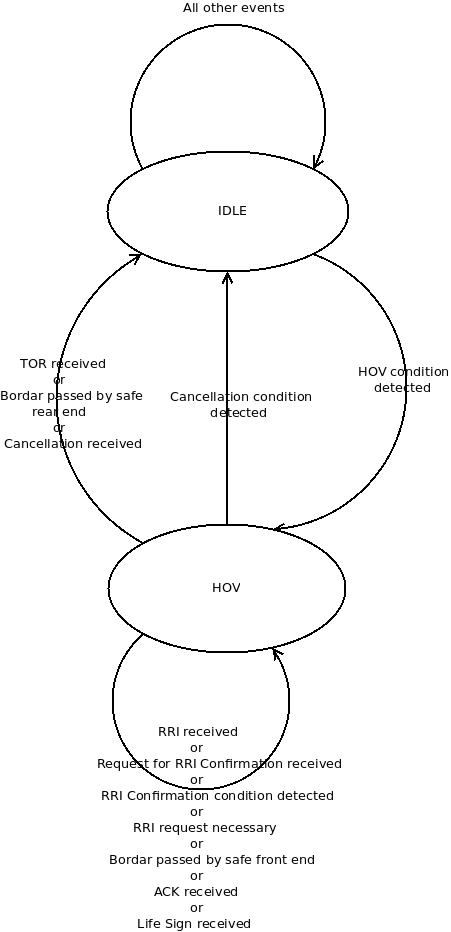
\includegraphics[width=8cm, height=8cm]{RBCTypeProcess.png}
\end{center}

\end{frame}

%\begin{fra
%\frametitle{Overview Of Process Algebra } % Table of contents slide, comment this block out to remove it
%
%\begin{itemize}
%\item ``Process algebra'' was initiated in 1982 by Bergstra and Klop \cite{begstraKlop:FixedPointSemantics}, in order to provide a formal semantics to concurrent systems
%
%\end{itemize}
%
%\begin{itemize}
%\item Baeten et.al :
% Process algebra is the study of distributed or parallel systems by algebraic means. \\~\\
%\begin{itemize}
%\item The word ‘process’ here refers to behavior of a system.
%\\~\\
%% A system is anything  showing behavior,  such as the
%% execution of a software system, the actions of a machine or even the actions of a human being.
%
%
%%Behavior is the total of events, actions or evolutions that a
%%system can perform, the order in which these can be executed and maybe other aspects of this execution such as timing, probabilities, or continuous  aspects.  
%%Always,  the focus is on certain aspects of behavior, disregarding  other aspects, so an abstraction or idealization of the ‘real’ behavior is considered
%
%%actions are usually thought to be discrete:  occurrence is at some moment in time, and different actions are separated in time.
%
%\item The word ‘algebra’ denotes that the approach in dealing with behavior is algebraic and axiomatic. \\~\\
%
%%A process algebra can be defined as any mathematical structure satisfying the axioms given for the basic operators
%
%\end{itemize}
%\item three main process algebra theories were developed.
%\begin{itemize}
%
%\item Calculus of Communicating Systems (CCS). \\
%{\footnotesize developed by Robin Milner in 1980}
%
%\item Communicating Sequential Processes (CSP). \\
%{\footnotesize developed by Tony Hoare in 1978  }
%
%\item Algebra of Communicating Processes (ACP). \\
%{\footnotesize developed by Jan Bergstra and Jan Willem Klop, in 1982 }
%
%\end{itemize}
%\end{itemize}
%\end{fram
%






% % % % % % % % % % % % % % % % % % % % % % % % % %

%CSP

% % % % % % % % % % % % % % % % % % % % % % % % % %





\begin{frame}
\frametitle {CSP}
\begin{itemize}

\item CSP considered as a formal specification language, developed in order to describe concurrent systems. \\
{\footnotesize By identifying their behaviour through their communications.}

\item CSP is a notation for studying processes which interact with each other and their environment.

\item In CSP we can describe a process by the way it can communicate with its environment. 

%The most fundamental object in CSP is an event, We call the set of events in CSP an alphabet, which contains all possible interaction for processes.

\item A system contains one or more processes, which interact with each other through their interfaces. 

\end{itemize}
\end{frame}




% % % % % % % % % % % % % % % % % % % % % % % % % %

%CSP operator

% % % % % % % % % % % % % % % % % % % % % % % % % %






\begin{frame}
\frametitle{CSP Syntax}
In the following table, we list the syntax of CSP processes:
\begin{center}
\begin{tabular}{p{2in}p{1.5in}c} 
 Q ::=
  STOP                            & $\ STOP   $           \\%[1ex]
  
 \hspace{25pt}$|$ SKIP            & $\ SKIP    $          \\%[1ex]
  
 \hspace{25pt}$|$ prefix          & $\ a \then Q $        \\%[1ex]
  
 \hspace{25pt}$|$ external choice & $\ Q \extchoice Q $   \\%[1ex]
  
 \hspace{25pt}$|$ internal choice & $\ Q \intchoice Q $   \\%[1ex]
  
 \hspace{25pt}$|$ hiding          & $\ Q \hide a $        \\%[1ex]

 \hspace{25pt}$|$ renaming        & $\ Q[R]      $        \\%[1ex]
  
 \hspace{25pt}$|$ parallel        & $\ Q \parallelWithIndices{X}{Y} Q $    \\
  
 \hspace{25pt}$|$ interleaving    & $\ Q \interleaveop Q $  \\%[1ex]
  
 \hspace{25pt}$|$ interrupt       & $\ Q \interrupt Q $   \\%[1ex]
  
 \hspace{25pt}$|$ composition     & $\ Q  ; Q $        \\%[1ex]
 
\end{tabular}
\end{center}
\end{frame}






%\begin{frame}
%\frametitle{Theorm prover Agda }
%\begin{itemize}
%
%\item Agda is a dependently typed functional programming language.
%
%\item The current version of this language is Agda2 which has been designed and implemented by Ulf Norell in his PhD in 2007.
%
%
%{\footnotesize Our work in this research  is carried out in the theorem prover Agda version 2.}
%
%
%\end{itemize}
%\begin{itemize}
%
%\item Agda language considered as a functional programming language with numerous features. 
%\begin{itemize}
%\item Total Language
%\begin{enumerate}
%\item Type checking % The Agda type checker refuses any incorrect proofs by detecting unmatched types.
%\item Coverage checking %in order to be sure that the patterns cover all possible cases
%\item Termination checking %Agda is a total language then each program in it must terminate, since Agda without termination checker makes the logic behind this language inconsistent.
%\item Strict positivity of constructors checking 
%\item Guardedness checking in coinductive programs
%%Needless to say, the most interesting challenges in the design of programming language is infinite coinductive data types and define function on them. Guarded corecursion considered as a kind of recursion which allowed arbitrary recursive calls as long as the are guarded by coinductive constructor.
%
%\end{enumerate}
%\item Undoubtedly Agda skilful supports pattern matching,
%\item Inductive Data Type 
%\item Mixfix Operators and Unicode 
%\item Interactive Interface
%
%\end{itemize}
%\end{itemize}
%\end{frame}




% % % % % % % % % % % % % % % % % % % % % % % % % %

%Over View 

% % % % % % % % % % % % % % % % % % % % % % % % % %






\begin{frame}
\frametitle{CSP-Agda}

\begin{itemize}

\item We will represent the process algebra CSP in a coinductive form in dependent type theory.

\item Implement it in the Agda.

\item CSP processes can proceed at any time both with labelled transitions and with silent transitions.

\item Therefore, processes in CSP-Agda have as well this possibility.
%\item  The first ones correspond to external choice and the latter correspond to internal choices.


\end{itemize}
\end{frame}




\begin{frame}
\frametitle{CSP-Agda}

In Agda the corresponding code is as follows: % assuming $\Label: \Set $:

\[\begin{array}[t]{@{}l} 
\record\ \Process: \Set\ \ \wheresf  \\
\mbox{\quad}
\begin{array}[t]{@{}lcl} 
\coinductive \\
\field \\
\mbox{\quad} \begin{array}[t]{@{}l}
\begin{array}[t]{@{}clclcl}
 & \e  &:& \Choice \\
 & \lab  &:&  \ChoiceSet \;\e &\ar& \Label\\
 & \pe   &:& \ChoiceSet\;\e &\ar& \Process\\
 & \ii    &:&  \Choice\\
 & \pii   &:&  \ChoiceSet \;\ii  &\ar& \Process\\

\end{array} 
\end{array} 
\end{array} 
\end{array} \]


\end{frame}


\begin{frame}
\frametitle{CSP-Agda}
So we have in case of a process progressing: 
\begin{itemize}

\item an index set $\e$ of external choices and for each external choice $e$ a label ($\lab\;e$) and a next process ($\pe\;e$);

\item an index set of internal choices $\i$ and for each internal choice $i$ a next process ($\pii\;i$ ).
\end{itemize}
\end{frame}







\begin{frame}
\frametitle{CSP-Agda}

As an example the following Agda code describes the process pictured below:
\[\begin{array}{@{}l@{}lclcl@{}lclcl@{}lcllclclclclclclclclcl}
\e \; &P &=& \multicolumn{25}{@{}l}{\mbox{code for }\{1,2,3\} 
\mbox{\qquad \qquad \qquad \qquad \qquad \qquad \qquad }}\\
\lab \; &P \;1 &=& a &\ & \lab \;&P\;2 &=& b & & \lab\; &P\;3 &=& c\\
\pe \; &P\;1 &=& P_1&  &\pe \; &P\;2 &=& P_2 & & \pe\; &P \;3 &=& P_3&
\\
\ \\
\ii\;&P&=& \multicolumn{25}{@{}l}{\mbox{ code for } \{4,5\}}\\
\pii \;&P\;4 &=& P_4&  &\pii \;&P\;5 &=& P_5
\end{array} \]

\includeXfigPictexWithoutFigure{exampleProcess}
\end{frame}



\begin{frame}
\frametitle{Choices Set}
\begin{itemize}

%\item We needed  to have a set of choices.
\item Choice sets are modelled by a universe. 

\item Universes go back to Martin-L{\"o}f in order to formulate the notion of a type consisting of types.

\item Universes are defined in Agda by an inductive-recursive definition.

%we define inductively the set of codes in the universe while
%recursively defining the decoding function.



\end{itemize}
\end{frame}





\begin{frame}
\frametitle{Choices Set}

We give here the code expressing that Choice is closed under $\Bool$, disjoint union $+$ and $\subsett$.

%Closure under other sets needed can be easily added as needed
%(the symbols for $\Boolhat$, $\plushat$ will be written as 
%$\Bool'$, $+'$ in actual Agda)


\[\begin{array}[t]{@{}l} 
\mutual\\
\mbox{\quad}
\begin{array}[t]{@{}l} 
\datarm\;\Choi : \Set\ \ \wheresf\\
\mbox{\quad} \begin{array}[t]{@{}lcl} 
\Boolhat &: & \Choi\\
\_\plushat\_ &:& \Choi \ar \Choi \ar \Choi\\
\subsett &:& (E : \Choi) \ar  (\ChoiceSet\; E \ar \Bool) \ar \Choi
\end{array} \end{array} \\
\\
\ChoiceSet : \Choice  \ar \Set \\
\begin{array}[t]{@{}lcl} 
\ChoiceSet\;\Boolhat &=& \Bool\\
\ChoiceSet\;(a \plushat b) &=& 
\ChoiceSet\;a + \ChoiceSet\;b \\
\ChoiceSet\;(\subsett\; E\; f) &=& \Subsett\; (\ChoiceSet\; E)\; f

\end{array} 
\end{array} 
\]

\end{frame}





%\begin{frame}
%\begin{itemize}
%\item In mathematical notation a process is represented as
%follows (assuming a set of labels $\Label:\Set$):
%\end{itemize}
%
%
%\[\begin{array}[t]{@{}l} 
%\Process = 
%\begin{array}[t]{@{}l@{}l} %\{&\terminate(a) \mid a \in A \}\; \cup\\
%\{&\node \;(E,\lab,\pe,I,\pii) \mid \begin{array}[t]{@{}l@{\;}c@{\;}ll@{\;}c@{\;}ll@{\;}c@{\;}ll@{\;}c@{\;}l}
%\; E &\in&\Choice,\\&
%\lab &:& E \ar \Label,\\&
%\pe  &:& E \ar \Process,\\&
%I   &\in& \Choice,\\&
%\pii  &:& \multicolumn{4}{l}{I \ar \Process\ \; \}}
%\end{array} \end{array} \end{array} \]
%
%\end{frame}
%

\begin{frame}
\frametitle{Interleaving operator}

\begin{itemize}

%\item Concurrent execution of processes P and Q where no such synchronization is described by the combination $ P \;\interleaveop\; Q$

\item In this process, the components P and Q execute completely
independently of each other.

\item Each event is performed by exactly one process. 

\item The operational semantics rules are straightforward:
\end{itemize}

\begin{center}
\begin{tabular}{ll}
\AxiomC{$P  \trans[l] \bar{P}$}
%\RightLabel{$[\ \mu \in \sigma \cup \tau ]$}
\UnaryInfC{$P \interleaveop Q  \trans[l] \bar{P} \interleaveop Q$}
\noLine
\UnaryInfC{}
\DisplayProof{}
&
\AxiomC{$Q  \trans[l] \bar{Q}$}
%\RightLabel{$[\ \mu \in \sigma \cup \tau ]$}
\UnaryInfC{$P \interleaveop Q  \trans[l] {P} \interleaveop \bar{Q}$}
\noLine
\UnaryInfC{}
\DisplayProof{}

\end{tabular}
\end{center}

\end{frame}




\begin{frame}
\frametitle{Interleaving operator }

We represent interleaving operator in CSP-Agda as follows

\[\begin{array}[t]{@{}lclclcl} 
\interleaveDef &\multicolumn{4}{l}{: \Process \; \ar\; \Process \; \ar \; \Process}\\
 \e   &(P\interleaveop Q)& &=& \e\; P\; +'\; \e\; Q \\
 \lab &(P\interleaveop Q)&\; (\inl\; x)&=& \lab\; P\; x \\
 \lab &(P\interleaveop Q)&\; (\inr\; x)&=& \lab\; Q\; x \\
 \pe &(P\interleaveop Q)&\; (\inl\; x)&=& \pe \; P\;\;x \interleaveop Q\\
 \pe  &(P\interleaveop Q)&\; (\inr\; x)&=& P  \interleaveop  \pe\; Q\;x   \\
 \ii   &(P\interleaveop Q)&\           &=& \ii  \; P\; +' \;\ii\; Q \\
 \pii  &(P\interleaveop Q)&\; (\inl\; x)&=& \pii \; P\;\;x \interleaveop Q  \\
 \pii  &(P\interleaveop Q)&\; (\inr\; x)&=& P \interleaveop \pii\; Q \;x \  \\
\end{array} \]

\end{frame}



%
%
%\begin{frame}
%\begin{itemize}
%\item The recursive references to $(\Process\;A)$ are labelled by $\infty$ to indicate that they are indeed coinductive, so infinite (in general non-well-founded) loops are allowed
%
%\end{itemize}
%\end{frame}


\begin{frame}
\frametitle{Traces}

\[\begin{array}[t]{@{}lcl} 
\datarm \Tr  : \List\;\Label \ar \Process  \ar \Set \ \  \wheresf \\
\mbox{\quad} \begin{array}[t]{lc@{}ll@{\;}c@{\;}l}
\emptyC &:& \multicolumn{4}{l}{\{ P : \Process \; \}} \\
&&\ar &\multicolumn{3}{l}{ \Tr \; [\,] \; P }\\
\extChoice  &:&\multicolumn{4}{l}{ \{ P : \Process \; \}} \\
&&\ar&  (x &:& \ChoiceSet\; (\e \; P )) \\
&&\ar &(l &:& \List\;\Label) \\
&&\ar &\multicolumn{3}{l}{\Tr \; l \; (\pe\; P \; x)} \\
&&\ar &\multicolumn{3}{l}{\Tr\; (\lab\; P\; x\; ::\; l)\; P}\\
\intChoice &:& \multicolumn{4}{l}{ \{ P : \Process  \}} \\
&& \ar  &(x &:& \ChoiceSet\; (\ii  \; P)) \\
&& \ar &(l &:& \List\;\Label)\\
&& \ar &\multicolumn{3}{l}{\Tr \; l \; (\pii\; P\; x) }\\
&& \ar &\multicolumn{3}{l}{\Tr\;l \; P} 
\end{array} 
\end{array} \]

\end{frame}


\begin{frame}
\frametitle{Traces Refinement}

The refinement relation $\refinedby_T$ on process is defined by 
\begin{center}
$P\refinedby_T Q$\\
if and only if \\
$\mathrm{traces}(Q)\subseteq \mathrm{traces}(P)$
\end{center}
%
%A process $\bar{P}$ is a trace refinment of $P\;$ $iff\;$ all the possible sequance of commuincation which $\bar{P}$ can do are also possible fo $P$. 
\begin{itemize}

\item The subscript $T$ indicates that we are working with traces.
The Agda definition is as follows:

\end{itemize}

\[\begin{array}[t]{@{}lcl} 
\_\refinedby_T\_ :\; (P\;: \Process \; ) \ar(P'\;: \Process \; )\ar \Set  \\
P \;\refinedby_T \;P' \; = (l : \List \; \Label) \ar \Tr \; l \; P' \ar \Tr \; l \; P\\



\end{array} \]



\end{frame}


\begin{frame}

\frametitle{ Proving Symmetry of Interleaving operator }


\[\begin{array}[t]{@{}l@{\,}l@{\,}l@{\,}l@{\,}l@{\,}l@{\,}l@{\,}c@{\,}l@{\,}l@{\,}l@{\,}l@{\,}l@{\,}l@{\,}l} 
\multicolumn{15}{@{}l}{\Sym|||  : (P\; Q\; :\; \Process) \; \ar\; (P \; ||| \; Q) \; \refinedby \; (Q \; ||| \; P) }  \\
  \Sym|||&P& Q &\multicolumn{4}{l}{\emptyC }&=&\multicolumn{4}{@{}l}{\emptyC} \\ 
  \Sym|||&P&Q&(\extChoice  &(\inl\; x)  &l  &tr)& =&\extChoice  &(\inr\; x)  &l   &(\Sym|||\; P\; (\pe\; Q\; x)&tr) \mbox{\qquad \qquad \qquad \qquad \qquad \qquad \qquad \qquad  }\\
 \Sym|||&P&Q& (\extChoice &(\inr\; x)  &l  &tr)&=&\extChoice  &(\inl\; x)  &l  &(\Sym|||\; (\pe\; P\; x)\; Q &tr)  \\
 \Sym|||&P&Q& (\intChoice  &(\inl\; x)  &l  &tr)& =& \intChoice & (\inr\; x)& l  &(\Sym|||\; P\; (\pii\; Q\; x) &tr)  \\
 \Sym|||&P&Q& (\intChoice\; &(\inr\; x)  &l  &tr)& =& \intChoice  &(\inl\; x)  &l  &(\Sym|||\; (\pii\; P\; x)\; Q &tr) \\
 
\end{array} \]

\end{frame}




%
%
%\begin{frame}
%\frametitle{Why Agda ... }
%\begin{itemize}
%
%
%
%\item Coq have a lot of features and tactics, \\ {\footnotesize for instance setoid rewrite, the program framework,type classes, omega, etc.} \\
%this tactics and feature are useful in order to write hard proofs in Coq. whereas Agda such features need to write by hand, and this useful to find solutions that fit for some problem domain. In comparison Agda is not tactic-based like Coq.
%
%
%
%\end{itemize}
%\end{frame}
%

\begin{frame}[fragile] 
\frametitle{Future Work }

\begin{itemize}
\item Looking to the future, we would like to model complex systems in Agda.
\item Model examples of processes occurring in the European Train Management System (ERTMS) in Agda. 
\item Show correctness. 
\end{itemize}

	

\end{frame}



\begin{frame}[fragile] 
\frametitle{Further Work }


\begin{itemize}


\item The other operations (external choice, internal choice, parallel operations, hiding, renaming, etc.)
are defined in a similar way.

\item  Several laws of CSP have been shown with respect to traces semantics and bisimulation.

\item A simulator of CSP processes in Agda has been developed. 
 

\item Define approach using Sized types.

\item For complex examples (e.g recursion) sized types are used to allow application of functions to the co-IH.
\end{itemize}
\end{frame}



%------------------------------------------------

\begin{frame}
\frametitle{Conclusion}
\begin{itemize}
\item  A formalisation of CSP in Agda has been developed using coalgebra types and copattern matching.  

\item We have shown CSP-Agda supports refinement proofs over CSP traces model.
\end{itemize}
\end{frame}








%------------------------------------------------

\bibliographystyle{abbrv}
\bibliography{TypePresentation.bib}
%------------------------------------------------

\begin{frame}
\Huge{\centerline{The End}}
\end{frame}


\end{document} 
